\chapter{Cluster distortion and bipolaron formation}
\label{chap:ground}

As discussed in section \ref{sec:lattice-distortions}, from the ground state of the model hamiltonian (\ref{eq:full-hamiltonian}) we can calculate, using (\ref{eq:dvsuir}), the difference in bond distances in the CuO$_2$ cluster for different values of the coupling parameter $\lambda_{ir}$.
First, in section \ref{sec:grd-phonon-proj} of this chapter, we reproduce the previous work by Mustre de Le\'{o}n \textit{et al.} \cite{MustredeLeon1992} which, from a similar calculation, determined that the relevant couplings are in the intermediate regime. Furthermore we present a more detailed analysis of the dependende of this cluster distortion with the coupling $\lambda_{ir}$ and show that it is dynamical only in a narrow coupling range.

Subsequently we turn our attention to the bipolaron binding energy. 
We can identify the difference between the ground state energy in the absence of electron-lattice interaction ($\lambda_{ir}=0$) and its value for the coupling value where this polaronic behaviour sets in as the bipolaron binding enerygy.
In section \ref{sec:grd-binding-energy} we calculate this binding energy comparing it with experimental results.
We also calculate the isotopic shift, as defined in (\ref{eq:isot-shift-def-grd}), for the oxygen substitution$^{16}$O$\rightarrow ^{18}$O as a function of $\lambda_{ir}$.

% Why we care about the polaron-tunneling state? (first ir-excitation) 

From \cite{Conradson1990}

The motion of the O(4) atom in the deep, double well potential $V(z)$ can be described by a two-level Hamiltonian $H=(\omega_T/2)\sigma_z$,  such that $H\ket{A}=+(\omega_T/2)\ket{A}$ and $H\ket{S}=-(\omega_T/2)\ket{S}$, where $\sigma_z$ is a Pauli spin matrixm and $\ket{S},\ket{A}$ denote the (symmetric) ground state and (antisymmetric) first excited state, respectively, separated by an energy $\hbar\omega_T=\hbar\omega_1-\hbar\omega_0$.

% Paraphrasing



\section{Cu(1)-O(4) local distortion}
\label{sec:grd-phonon-proj}

The wavefunction projection into phonon coordinates (\ref{eq:phonon-coord-projection}) gives information about the coodinates of the three atoms in the CuO$_2$ cluster.
In particular, the phonon coordinate\footnote{The phonon coordinates are  defined in (\ref{eq:uR}, \ref{eq:uir}).} $u_{ir}$ is directly proportional to the distance distortion in the CuO$_2$ cluster, $d$, as shown in (\ref{eq:dvsuir}).
Figure \ref{fig:ph-ground} shows the ground state projected into phonon coordinates $(u_R,u_{ir})$ for three representative electron-lattice coupling values $\lambda_{ir}=0, 0.13$ and 0.25 eV.
The projection along $u_R$ is harmonic in all cases.
From the $\lambda_{ir}=0$ case the wavefunction's projection has a maximum at $u_{ir}=0$ impliying, as expected, there is no distortion in the cluster.
In the middle coupling regime, exemplified in Fig. \ref{fig:ph-ground} by $\lambda_{ir}=0.13$ eV, there are clearly two peaks present although they are not fully separated.
Since the probability amplitude is not neglible between the two maxima the system can \textit{tunnel} between both possible configurations with the longer distance in the first oxygen or the second bond.
This observation can be interpreted as a dynamic distortion in the cluster that can only be experimentally identifyied with a technique with a similar timescale (see discussion in secion \ref{sec:dynamic_dist}). 
For greater coupling values the two peaks are completely separated and the distortion becomes static.

\begin{figure}[ht!]
  \centering
  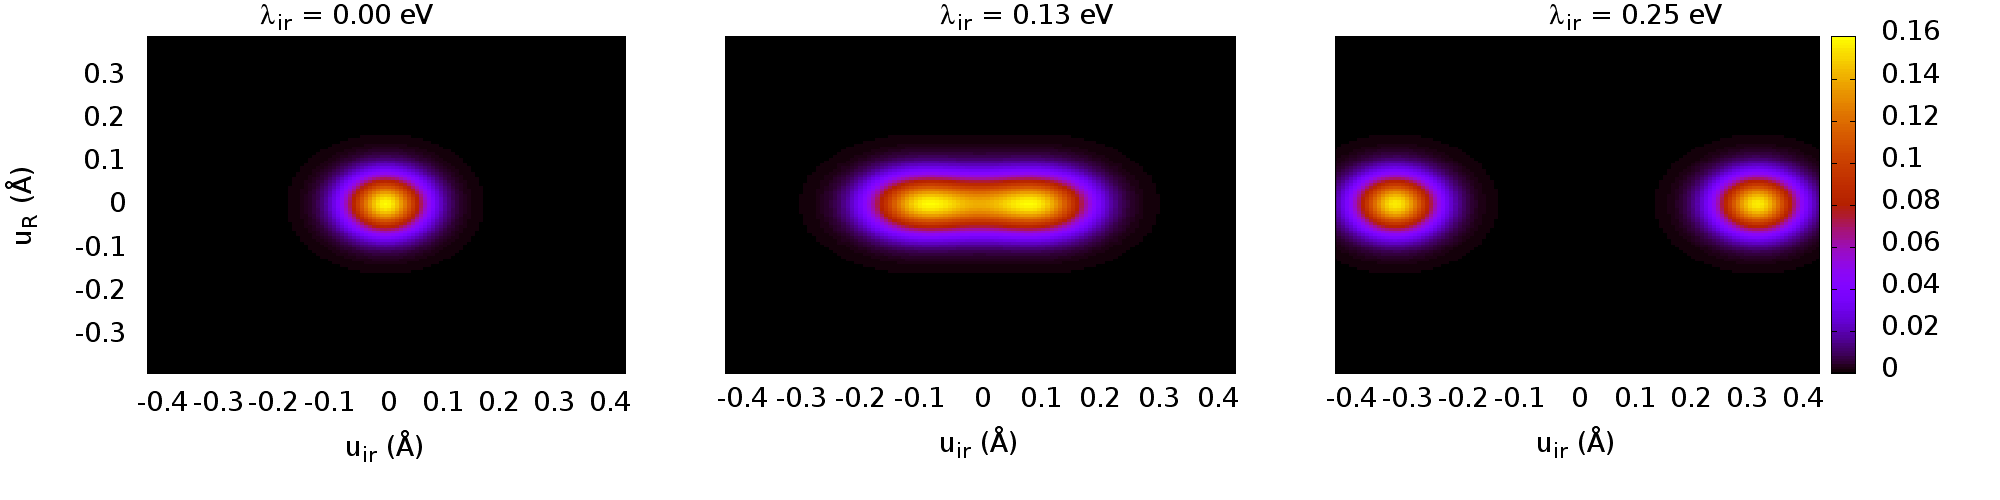
\includegraphics[width=1.0\textwidth]{images/ph-ground.png}
  \caption{Ground state's projection into phonon coordinates for three different values of the coupling parameter $\lambda_{ir}$.}
  \label{fig:ph-ground}
\end{figure}

Since the projection into $u_R$ does not change, giving that we are considering only $\lambda_R=0$, we calculated the projections with $u_R=0$ with variable $u_{ir}$ for different coupling values.
The left panel of figure \ref{fig:uir-vs-coupl} shows a plot of this comparison.
From here we can see that the distortion only sets in for $\lambda_{ir}$ greater than $\sim 0.12$ eV and becomes static (the two peaks are fully separated) for $\lambda_{ir}$ greater that $\sim 0.16$ eV.
In the right panel of figure \ref{fig:uir-vs-coupl} we show the cluster distortion $d$ calculated from the maxima of the previous projection.
Here we can see that the observed cluster distortion of $\sim 0.13$ \AA\ \cite{MustredeLeon1990} is reproduced in the intermedite coupling values. 
In particular, $\lambda_{ir}=0.1263$ eV reproduces that distortion.
From this plots we observe that it is only in the narrow range  $\sim 0.12 < \lambda_{ir} < \sim 0.16$ that a dynamical cluster distortion is present. 

\begin{figure}[ht!]
  \centering
  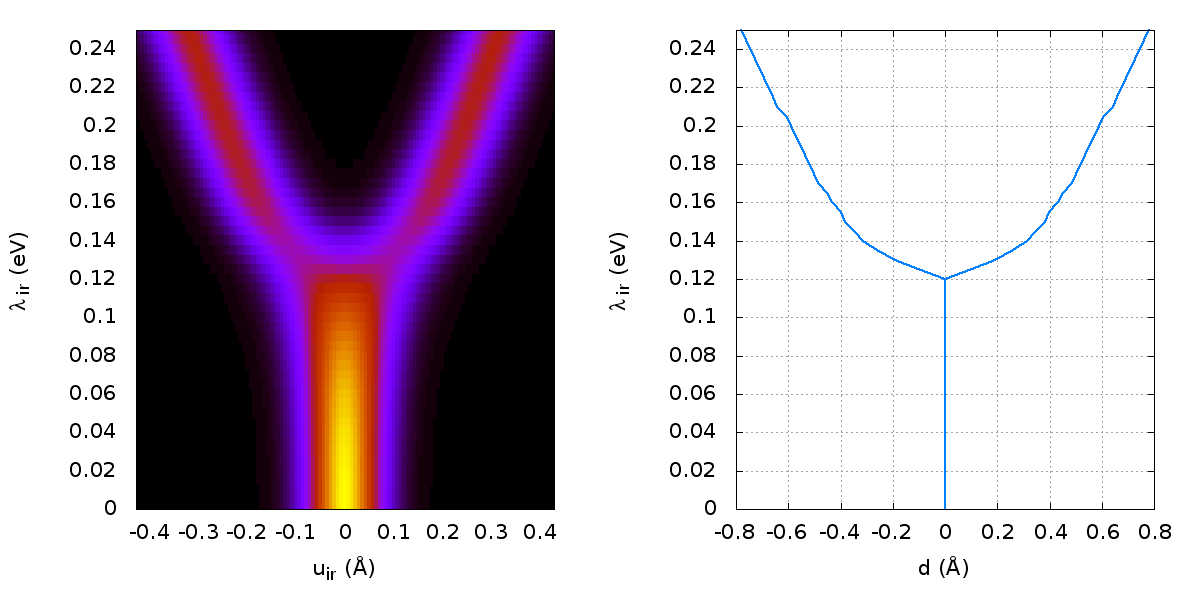
\includegraphics[width=1.0\textwidth]{images/uir-vs-coupl-d.png}
  \caption{Projection into phonon coordinates (left panel) and calculated cluster distortion $d$ (right panel) for different $\lambda_{ir}$ coupling values with $u_R=0$.}
  \label{fig:uir-vs-coupl}
\end{figure}

The polaron-tunneling energy $\hbar\omega_T$, at the relevant $\lambda_{ir}=0.1263$ eV is 141.39 cm$^{-1}$.

\section{Bipolaron binding energy}
\label{sec:grd-binding-energy}

The energy of the ground state changes with the coupling parameter $\lambda_{ir}$.
The change in energy, $\Delta\omega_{g}$, between the coupled and uncoupled systems can be identified as the \textit{formation energy}.
In particular, in the region where there is bipolaronic objects present, $\Delta\omega_{g}$ can be interpreted as the \textit{bipolaron binding energy}. 
In figure \ref{fig:polaronFormation} we show the dependency of $\Delta\omega_{g}$ with $\lambda_{ir}$, where we defined

\begin{equation}
  \label{eq:pol-energy}
  \Delta\omega_{g}(\lambda_{ir}) = \omega_{g}(\lambda_{ir} = 0) - \omega_{g}(\lambda_{ir})
\end{equation}

\begin{figure}
  \centering
  % GNUPLOT: LaTeX picture with Postscript
\begingroup
  \makeatletter
  \providecommand\color[2][]{%
    \GenericError{(gnuplot) \space\space\space\@spaces}{%
      Package color not loaded in conjunction with
      terminal option `colourtext'%
    }{See the gnuplot documentation for explanation.%
    }{Either use 'blacktext' in gnuplot or load the package
      color.sty in LaTeX.}%
    \renewcommand\color[2][]{}%
  }%
  \providecommand\includegraphics[2][]{%
    \GenericError{(gnuplot) \space\space\space\@spaces}{%
      Package graphicx or graphics not loaded%
    }{See the gnuplot documentation for explanation.%
    }{The gnuplot epslatex terminal needs graphicx.sty or graphics.sty.}%
    \renewcommand\includegraphics[2][]{}%
  }%
  \providecommand\rotatebox[2]{#2}%
  \@ifundefined{ifGPcolor}{%
    \newif\ifGPcolor
    \GPcolortrue
  }{}%
  \@ifundefined{ifGPblacktext}{%
    \newif\ifGPblacktext
    \GPblacktextfalse
  }{}%
  % define a \g@addto@macro without @ in the name:
  \let\gplgaddtomacro\g@addto@macro
  % define empty templates for all commands taking text:
  \gdef\gplbacktext{}%
  \gdef\gplfronttext{}%
  \makeatother
  \ifGPblacktext
    % no textcolor at all
    \def\colorrgb#1{}%
    \def\colorgray#1{}%
  \else
    % gray or color?
    \ifGPcolor
      \def\colorrgb#1{\color[rgb]{#1}}%
      \def\colorgray#1{\color[gray]{#1}}%
      \expandafter\def\csname LTw\endcsname{\color{white}}%
      \expandafter\def\csname LTb\endcsname{\color{black}}%
      \expandafter\def\csname LTa\endcsname{\color{black}}%
      \expandafter\def\csname LT0\endcsname{\color[rgb]{1,0,0}}%
      \expandafter\def\csname LT1\endcsname{\color[rgb]{0,1,0}}%
      \expandafter\def\csname LT2\endcsname{\color[rgb]{0,0,1}}%
      \expandafter\def\csname LT3\endcsname{\color[rgb]{1,0,1}}%
      \expandafter\def\csname LT4\endcsname{\color[rgb]{0,1,1}}%
      \expandafter\def\csname LT5\endcsname{\color[rgb]{1,1,0}}%
      \expandafter\def\csname LT6\endcsname{\color[rgb]{0,0,0}}%
      \expandafter\def\csname LT7\endcsname{\color[rgb]{1,0.3,0}}%
      \expandafter\def\csname LT8\endcsname{\color[rgb]{0.5,0.5,0.5}}%
    \else
      % gray
      \def\colorrgb#1{\color{black}}%
      \def\colorgray#1{\color[gray]{#1}}%
      \expandafter\def\csname LTw\endcsname{\color{white}}%
      \expandafter\def\csname LTb\endcsname{\color{black}}%
      \expandafter\def\csname LTa\endcsname{\color{black}}%
      \expandafter\def\csname LT0\endcsname{\color{black}}%
      \expandafter\def\csname LT1\endcsname{\color{black}}%
      \expandafter\def\csname LT2\endcsname{\color{black}}%
      \expandafter\def\csname LT3\endcsname{\color{black}}%
      \expandafter\def\csname LT4\endcsname{\color{black}}%
      \expandafter\def\csname LT5\endcsname{\color{black}}%
      \expandafter\def\csname LT6\endcsname{\color{black}}%
      \expandafter\def\csname LT7\endcsname{\color{black}}%
      \expandafter\def\csname LT8\endcsname{\color{black}}%
    \fi
  \fi
  \setlength{\unitlength}{0.0500bp}%
  \begin{picture}(6802.00,3968.00)%
    \gplgaddtomacro\gplbacktext{%
      \colorrgb{0.31,0.31,0.31}%
      \put(946,751){\makebox(0,0)[r]{\strut{}-600}}%
      \colorrgb{0.31,0.31,0.31}%
      \put(946,1235){\makebox(0,0)[r]{\strut{}-500}}%
      \colorrgb{0.31,0.31,0.31}%
      \put(946,1719){\makebox(0,0)[r]{\strut{}-400}}%
      \colorrgb{0.31,0.31,0.31}%
      \put(946,2203){\makebox(0,0)[r]{\strut{}-300}}%
      \colorrgb{0.31,0.31,0.31}%
      \put(946,2687){\makebox(0,0)[r]{\strut{}-200}}%
      \colorrgb{0.31,0.31,0.31}%
      \put(946,3171){\makebox(0,0)[r]{\strut{}-100}}%
      \colorrgb{0.31,0.31,0.31}%
      \put(946,3655){\makebox(0,0)[r]{\strut{} 0}}%
      \colorrgb{0.31,0.31,0.31}%
      \put(1125,484){\makebox(0,0){\strut{} 0}}%
      \colorrgb{0.31,0.31,0.31}%
      \put(2181,484){\makebox(0,0){\strut{} 0.05}}%
      \colorrgb{0.31,0.31,0.31}%
      \put(3237,484){\makebox(0,0){\strut{} 0.1}}%
      \colorrgb{0.31,0.31,0.31}%
      \put(4293,484){\makebox(0,0){\strut{} 0.15}}%
      \colorrgb{0.31,0.31,0.31}%
      \put(5349,484){\makebox(0,0){\strut{} 0.2}}%
      \colorrgb{0.31,0.31,0.31}%
      \put(6405,484){\makebox(0,0){\strut{} 0.25}}%
      \csname LTb\endcsname%
      \put(176,2227){\rotatebox{-270}{\makebox(0,0){\strut{}$\Delta\omega_g (meV)$}}}%
      \put(3765,154){\makebox(0,0){\strut{}$\lambda_{ir}$ (eV)}}%
      \put(3871,1105){\makebox(0,0)[l]{\strut{}\scriptsize$\lambda_{ir}=0.1263$}}%
    }%
    \gplgaddtomacro\gplfronttext{%
    }%
    \gplbacktext
    \put(0,0){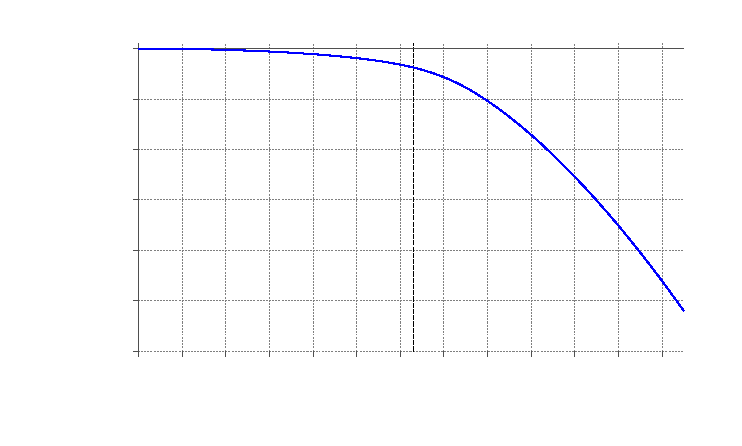
\includegraphics{images/polaronFormation}}%
    \gplfronttext
  \end{picture}%
\endgroup

  \caption{Bipolaron formation energy as a function of the $\lambda_{ir}$ coupling. The vertical line is drawn at the relevant value $\lambda_{ir}=0.1263$ eV.}
  \label{fig:polaronFormation}
\end{figure}

We observe a monotonical behaviour with small dependency in the weak coupling regime becoming stronger with greater coupling values.
In particular, for the $\lambda_{ir}=0.1263$ eV value, which reproduces the observed distortion, we find $\Delta\omega_{g}(0.1263$ eV$) = \sim 38$ meV.
This value compares favorably with the value obtained from femtosecond time-domain spectroscopy ($\sim 45$ meV) for YBa$_2$Cu$_3$O$_7$ \cite{Demsar1999}. 
We also find that if we consider a smaller electron-lattice coupling such that the distortion is 0.08 \AA, as that observed for in plane Cu(2)-O in La$_{1.85}$Sr$_{0.15}$CuO$_4$ \cite{Bianconi1996}, we obtain $E_p \sim 35$ meV, which is also comparable to estimates for the pseudogap formation energy in this system (see Fig. 4b in \cite{Kusar2005}).

\section{Isotopic effects in bipolaron formation}
\label{sec:grd-isotopic}

We turn our attention now to the isotopic shift, $\Delta_g$, of $\omega_g$ under the $^{16}$O$\rightarrow ^{18}$O substitution as defined in (\ref{eq:isot-shift-def-grd}).
Figure \ref{fig:isotPolaronFormation} shows $\Delta_g$ as a function of $\lambda_{ir}$.
Contrary to other isotopic shifts, it does not change sign.
However it shows a maximum in the middle coupling regime, reminiscent of the maximums, minimums and inflection points in the isotopic shifts of all other excitations.

\begin{figure}[ht!]
  \centering
  % GNUPLOT: LaTeX picture with Postscript
\begingroup
  \makeatletter
  \providecommand\color[2][]{%
    \GenericError{(gnuplot) \space\space\space\@spaces}{%
      Package color not loaded in conjunction with
      terminal option `colourtext'%
    }{See the gnuplot documentation for explanation.%
    }{Either use 'blacktext' in gnuplot or load the package
      color.sty in LaTeX.}%
    \renewcommand\color[2][]{}%
  }%
  \providecommand\includegraphics[2][]{%
    \GenericError{(gnuplot) \space\space\space\@spaces}{%
      Package graphicx or graphics not loaded%
    }{See the gnuplot documentation for explanation.%
    }{The gnuplot epslatex terminal needs graphicx.sty or graphics.sty.}%
    \renewcommand\includegraphics[2][]{}%
  }%
  \providecommand\rotatebox[2]{#2}%
  \@ifundefined{ifGPcolor}{%
    \newif\ifGPcolor
    \GPcolortrue
  }{}%
  \@ifundefined{ifGPblacktext}{%
    \newif\ifGPblacktext
    \GPblacktextfalse
  }{}%
  % define a \g@addto@macro without @ in the name:
  \let\gplgaddtomacro\g@addto@macro
  % define empty templates for all commands taking text:
  \gdef\gplbacktext{}%
  \gdef\gplfronttext{}%
  \makeatother
  \ifGPblacktext
    % no textcolor at all
    \def\colorrgb#1{}%
    \def\colorgray#1{}%
  \else
    % gray or color?
    \ifGPcolor
      \def\colorrgb#1{\color[rgb]{#1}}%
      \def\colorgray#1{\color[gray]{#1}}%
      \expandafter\def\csname LTw\endcsname{\color{white}}%
      \expandafter\def\csname LTb\endcsname{\color{black}}%
      \expandafter\def\csname LTa\endcsname{\color{black}}%
      \expandafter\def\csname LT0\endcsname{\color[rgb]{1,0,0}}%
      \expandafter\def\csname LT1\endcsname{\color[rgb]{0,1,0}}%
      \expandafter\def\csname LT2\endcsname{\color[rgb]{0,0,1}}%
      \expandafter\def\csname LT3\endcsname{\color[rgb]{1,0,1}}%
      \expandafter\def\csname LT4\endcsname{\color[rgb]{0,1,1}}%
      \expandafter\def\csname LT5\endcsname{\color[rgb]{1,1,0}}%
      \expandafter\def\csname LT6\endcsname{\color[rgb]{0,0,0}}%
      \expandafter\def\csname LT7\endcsname{\color[rgb]{1,0.3,0}}%
      \expandafter\def\csname LT8\endcsname{\color[rgb]{0.5,0.5,0.5}}%
    \else
      % gray
      \def\colorrgb#1{\color{black}}%
      \def\colorgray#1{\color[gray]{#1}}%
      \expandafter\def\csname LTw\endcsname{\color{white}}%
      \expandafter\def\csname LTb\endcsname{\color{black}}%
      \expandafter\def\csname LTa\endcsname{\color{black}}%
      \expandafter\def\csname LT0\endcsname{\color{black}}%
      \expandafter\def\csname LT1\endcsname{\color{black}}%
      \expandafter\def\csname LT2\endcsname{\color{black}}%
      \expandafter\def\csname LT3\endcsname{\color{black}}%
      \expandafter\def\csname LT4\endcsname{\color{black}}%
      \expandafter\def\csname LT5\endcsname{\color{black}}%
      \expandafter\def\csname LT6\endcsname{\color{black}}%
      \expandafter\def\csname LT7\endcsname{\color{black}}%
      \expandafter\def\csname LT8\endcsname{\color{black}}%
    \fi
  \fi
  \setlength{\unitlength}{0.0500bp}%
  \begin{picture}(6802.00,3968.00)%
    \gplgaddtomacro\gplbacktext{%
      \colorrgb{0.31,0.31,0.31}%
      \put(726,751){\makebox(0,0)[r]{\strut{}\scriptsize 5}}%
      \colorrgb{0.31,0.31,0.31}%
      \put(726,1243){\makebox(0,0)[r]{\strut{}\scriptsize 6}}%
      \colorrgb{0.31,0.31,0.31}%
      \put(726,1735){\makebox(0,0)[r]{\strut{}\scriptsize 7}}%
      \colorrgb{0.31,0.31,0.31}%
      \put(726,2227){\makebox(0,0)[r]{\strut{}\scriptsize 8}}%
      \colorrgb{0.31,0.31,0.31}%
      \put(726,2719){\makebox(0,0)[r]{\strut{}\scriptsize 9}}%
      \colorrgb{0.31,0.31,0.31}%
      \put(726,3211){\makebox(0,0)[r]{\strut{}\scriptsize 10}}%
      \colorrgb{0.31,0.31,0.31}%
      \put(726,3703){\makebox(0,0)[r]{\strut{}\scriptsize 11}}%
      \colorrgb{0.31,0.31,0.31}%
      \put(905,484){\makebox(0,0){\strut{}\scriptsize 0}}%
      \colorrgb{0.31,0.31,0.31}%
      \put(2005,484){\makebox(0,0){\strut{}\scriptsize 0.05}}%
      \colorrgb{0.31,0.31,0.31}%
      \put(3105,484){\makebox(0,0){\strut{}\scriptsize 0.1}}%
      \colorrgb{0.31,0.31,0.31}%
      \put(4205,484){\makebox(0,0){\strut{}\scriptsize 0.15}}%
      \colorrgb{0.31,0.31,0.31}%
      \put(5305,484){\makebox(0,0){\strut{}\scriptsize 0.2}}%
      \colorrgb{0.31,0.31,0.31}%
      \put(6405,484){\makebox(0,0){\strut{}\scriptsize 0.25}}%
      \csname LTb\endcsname%
      \put(352,2227){\rotatebox{-270}{\makebox(0,0){\strut{}$\Delta_g\ (meV)$}}}%
      \put(3655,154){\makebox(0,0){\strut{}$\lambda_{ir}$ (eV)}}%
      \put(3765,1105){\makebox(0,0)[l]{\strut{}\scriptsize$\lambda_{ir}=0.1263$}}%
    }%
    \gplgaddtomacro\gplfronttext{%
    }%
    \gplbacktext
    \put(0,0){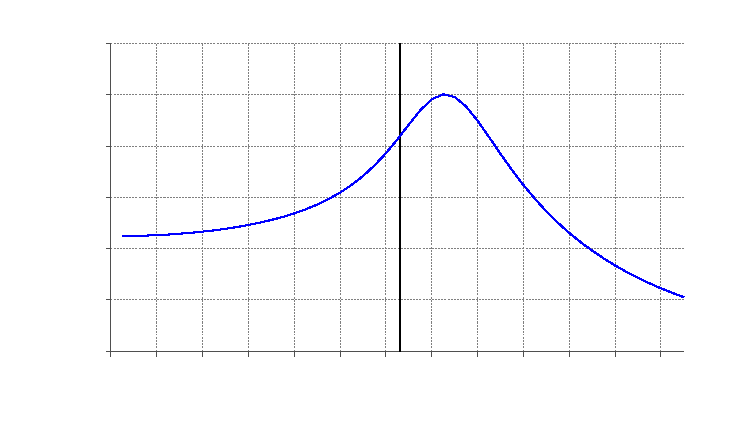
\includegraphics{images/isotPolaronFormation}}%
    \gplfronttext
  \end{picture}%
\endgroup

  \caption{Isotopic shift of the bipolaron formation energy. The vertical line is placed at the relevant value $\lambda_{ir}=0.1263$.}
  \label{fig:isotPolaronFormation}
\end{figure}

% Figure of projection into definite electron-occupation basis for both, the ground and polaron-tunneling state

\section{Polaron tunneling}

% Only the ground state and the first ir-excitation are appreciably occupied at the temperatures of interest thus the O(4) motion needs to be described quantum mechanically.
% prove? What is the energy difference (in Kelvin) between the ground state and all the excitations?
% in cite{MustredeLeon1992a} they call $\hbar \omega_T = \Delta\epsilon = \epsilon_1 - \epsilon_0 \sim 80$ K the ``interwell tunneling frequency''

% \hbar\omega_T is the tunneling frequency between the two minima

\section{Projection into phonon coordinates}

\begin{figure}[ht!]
\centering
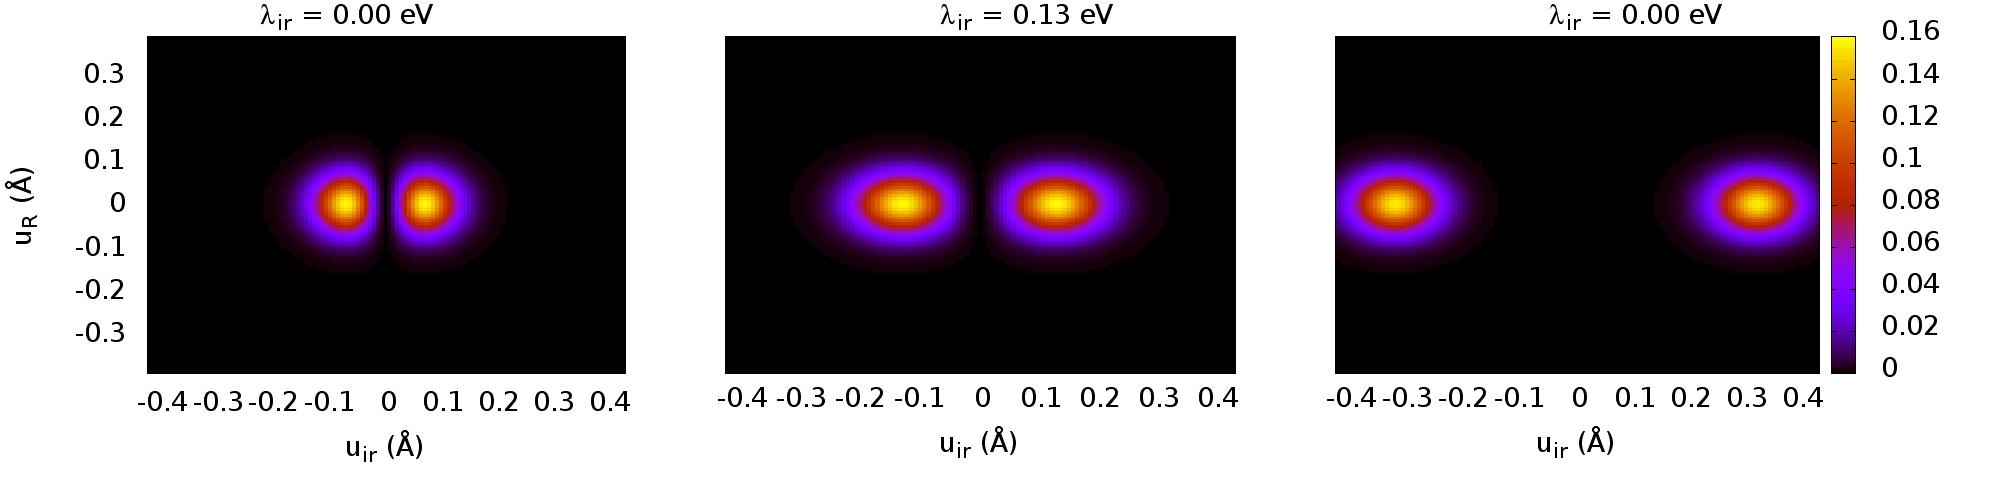
\includegraphics[width=0.8\textwidth]{images/ph-first_infrared.png}
\caption{Polaron tunneling state's projection into phonon coordinates.}
\label{fig:ph-first_infrared}
\end{figure}

\section{Isotopic shift}
\label{sec:polaron-isotopic-shift}

\begin{figure}[ht!]
\centering
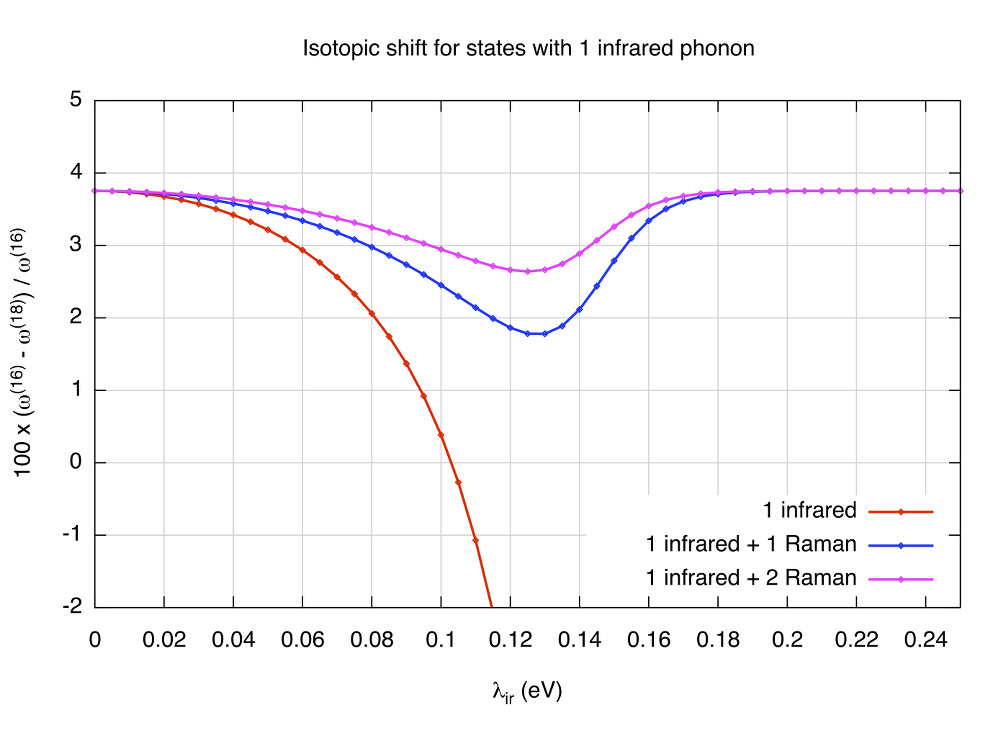
\includegraphics[width=0.8\textwidth]{images/isot-1ir.jpg}
\caption{Isotopic shift for the first infrared-allowed excitation.}
\label{fig:isot-1ir}
\end{figure}

